\documentclass[11pt]{standalone}
\usepackage{amssymb}
\usepackage{amsmath}
\usepackage[no-math]{fontspec}
\usepackage{unicode-math}
\usepackage{libertinus}
\usepackage{pgf,xcolor}
\usepackage{tikz}
\usetikzlibrary{arrows.meta, backgrounds}
\usepackage{pgfplots}
\pgfplotsset{compat=newest}

\setmainfont{Libertinus Serif}
\setmathfont{Libertinus Math}

\definecolor{my_darkgray}{HTML}{484949}
\definecolor{my_lightgray}{HTML}{F3F4F4}
\definecolor{my_darkblue}{HTML}{005A94}
\definecolor{my_lightblue}{HTML}{CCDEE9}
\definecolor{my_yellow}{HTML}{FFEC7F}
\definecolor{my_red}{HTML}{E60000}
\definecolor{my_orange}{HTML}{E87846}

\begin{document}

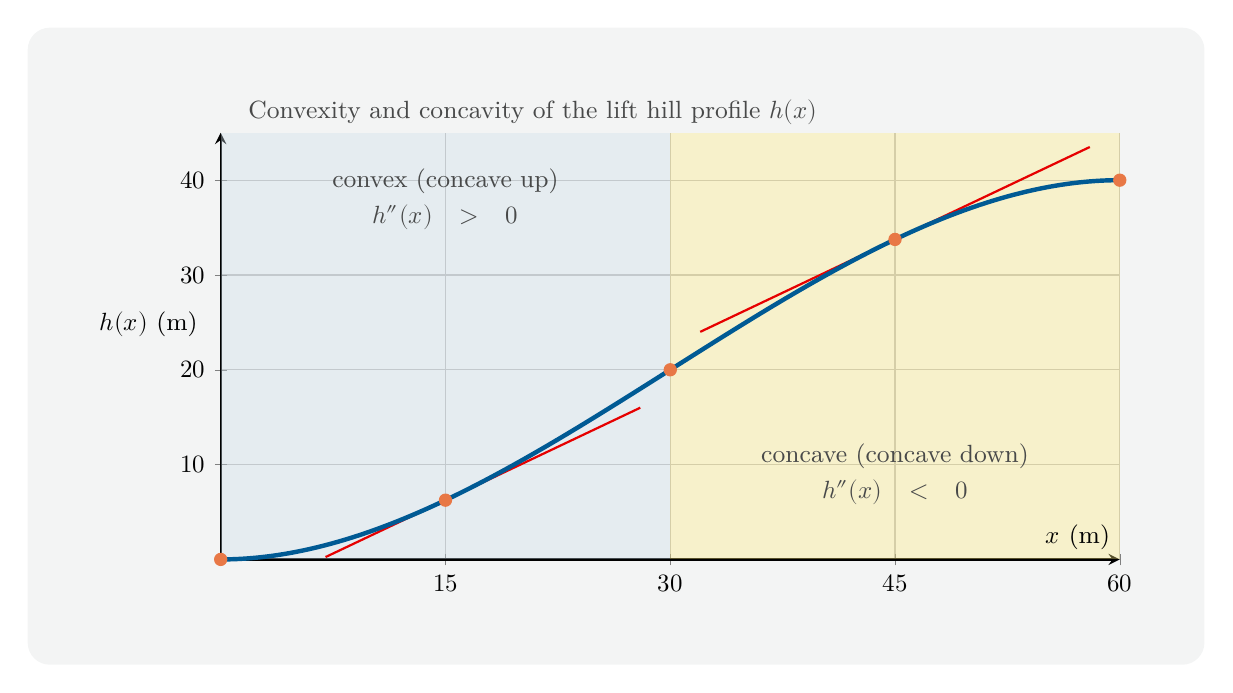
\begin{tikzpicture}[
    show background rectangle,
    background rectangle/.style={fill=my_lightgray, rounded corners=8pt},
    inner frame sep=0.8cm
]

\begin{axis}[
    width=13cm,
    height=7cm,
    axis lines = center,
    xlabel = {$x$ (m)},
    ylabel = {$h(x)$ (m)},
    xmin=0, xmax=60,
    ymin=0, ymax=45,
    xtick={0,15,30,45,60},
    ytick={0,10,20,30,40},
    grid = major,
    axis line style={thick},
    ticklabel style={font=\small},
    label style={font=\small},
    ylabel style={
      at={(axis description cs:-0.08,0.5)},
      anchor=south
    },
    clip=false,
]

% background shading: convex region [0, 30]
\fill[my_lightblue, opacity=0.35]
  (axis cs:0,0) rectangle (axis cs:30,45);

% background shading: concave region [30, 60]
\fill[my_yellow, opacity=0.35]
  (axis cs:30,0) rectangle (axis cs:60,45);

% tangent at x = 15: y = 0.75x - 5, drawn on [7, 28]
% at x=7: y=0.25; at x=28: y=16  -- both inside plot
\addplot[
    draw=my_red,
    thick,
    domain=7:28,
    samples=2
]
{0.75*x - 5};

% tangent at x = 45: y = 0.75x, drawn on [32, 58]
% at x=32: y=24; at x=58: y=43.5  -- both inside plot
\addplot[
    draw=my_red,
    thick,
    domain=32:58,
    samples=2
]
{0.75*x};

% lift hill height profile h(x) = x^2/30 - x^3/2700
% drawn on top of tangents so curve is always visible
\addplot[
    draw=my_darkblue,
    ultra thick,
    samples=400,
    domain=0:60
]
{0.0333333333*x^2 - 0.00037037037*x^3};

% five key points at x = 0, 15, 30, 45, 60
\addplot[
    only marks,
    mark=*,
    mark size=2.2pt,
    draw=my_orange,
    fill=my_orange
]
coordinates {
  (0,0)
  (15,6.25)
  (30,20)
  (45,33.75)
  (60,40)
};

% region label: convex -- placed at (9, 38), well above curve h(9) ≈ 2.4
\node[
    anchor=center,
    font=\small,
    my_darkgray,
    text width=5.5cm,
    align=center
]
at (axis cs:15,38)
{convex (concave up)\\[2pt]$h''(x) > 0$};

% region label: concave -- placed at (51, 9), well below curve h(51) ≈ 37.6
\node[
    anchor=center,
    font=\small,
    my_darkgray,
    text width=5.5cm,
    align=center
]
at (axis cs:45,9)
{concave (concave down)\\[2pt]$h''(x) < 0$};

% figure title, top-left inside plot
\node[
    anchor=north west,
    font=\small,
    my_darkgray
]
at (rel axis cs:0.02,1.1)
{Convexity and concavity of the lift hill profile $h(x)$};

\end{axis}

\end{tikzpicture}

\end{document}